%
\section{Interface}
\label{sec:lepton-interface}
The Raspberry Pi seen in section (\ref{sec:raspi3}) has bi-directional I/O pins, which you can use to drive LEDs, spin motors, or read button presses.
The board offers its GPIO over a standard male header on the board. Over the years the header has expanded from 26 pins to 40 pins while maintaining the original pinout.
There are at least two, different numbering schemes you may encounter when referencing pin numbers:
\begin{enumerate}
\item Broadcom chip-specific pin numbers 
\item \texttt{P1} physical pin numbers.
\end{enumerate} 
Here's a figure \ref{fig:gpio} showing all 26 pins on the \texttt{P1} header, including any special function they may have, and their dual numbers.
%
%
\begin{figure}[htb]
	\centering
	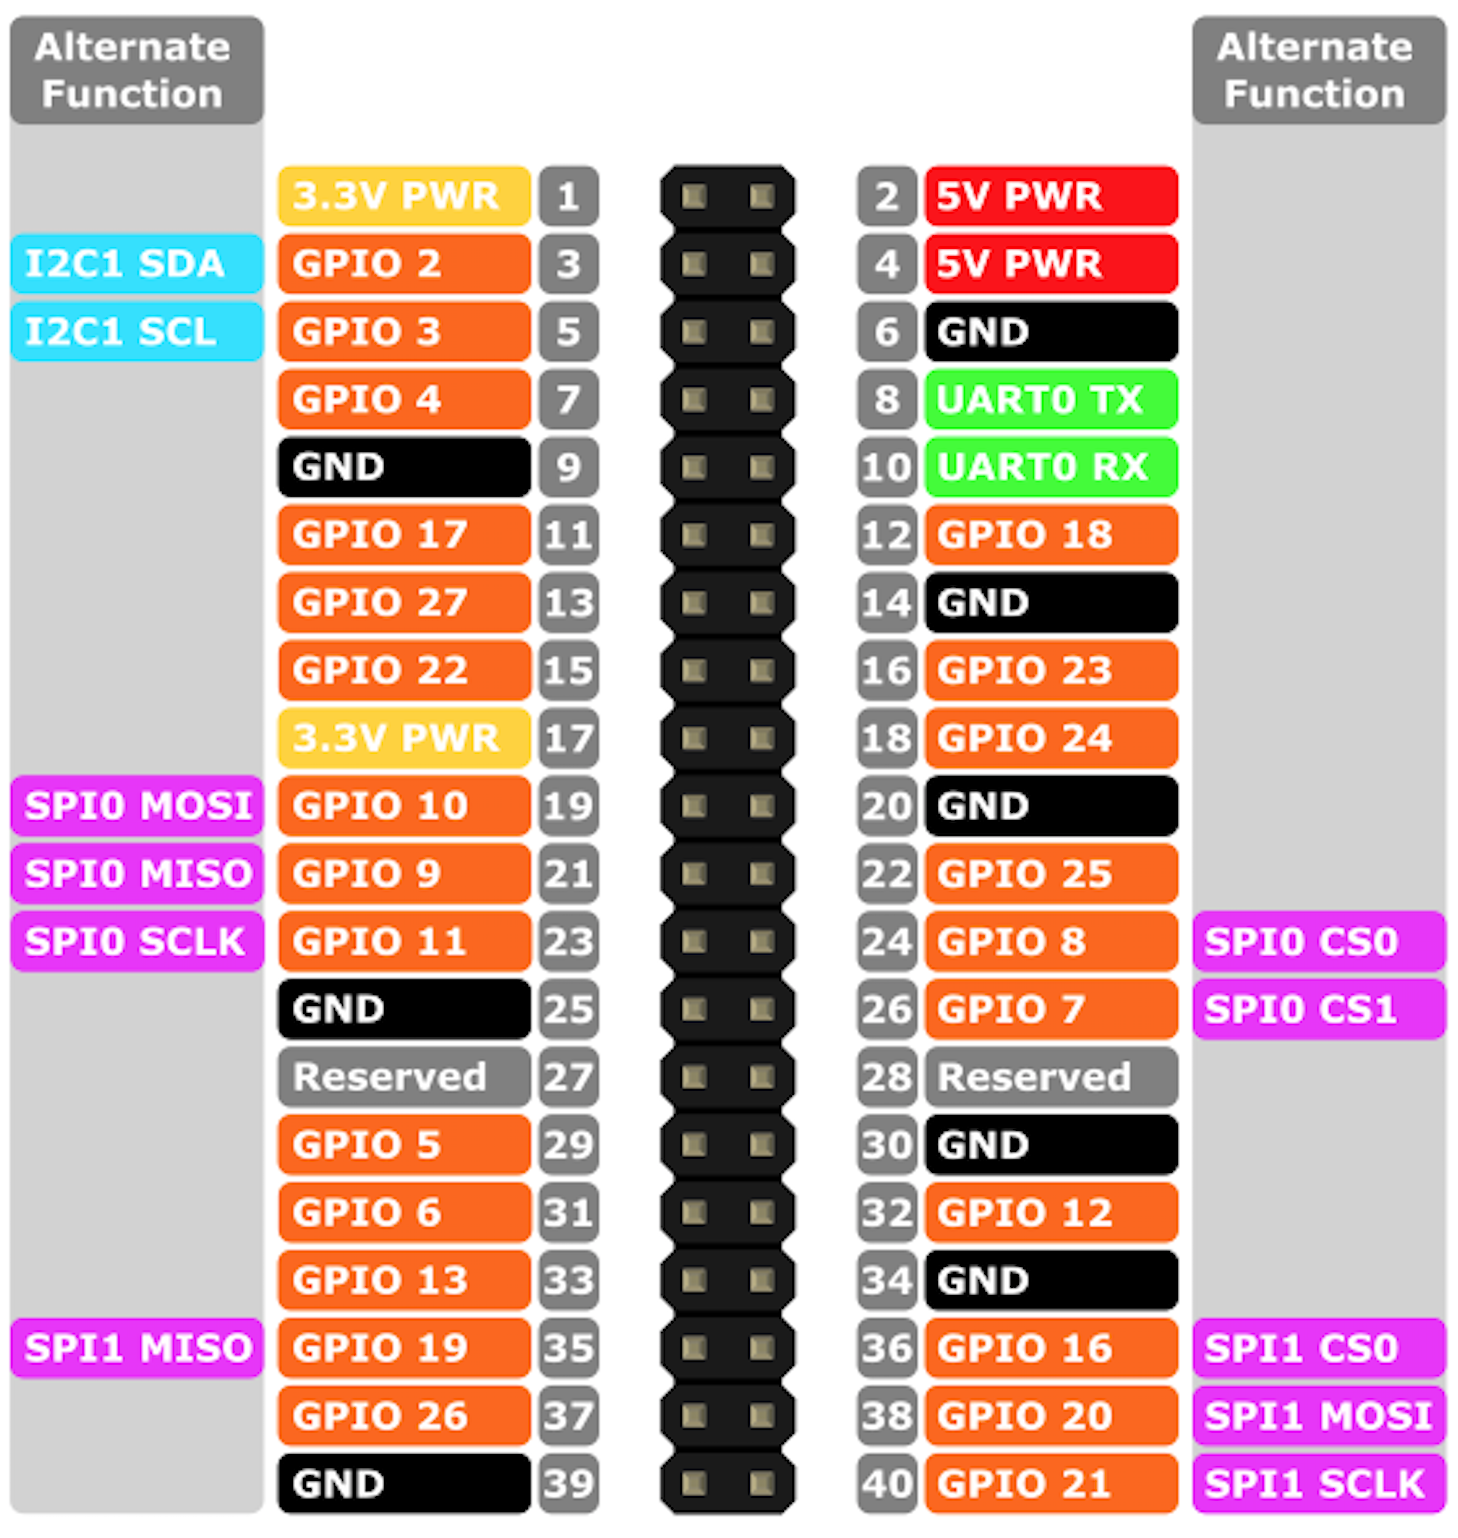
\includegraphics[width=0.45\textwidth]{gpio.png}
	\captionsource{Raspberry Pi 3 Pin Mappings.}{\href{https://docs.microsoft.com/es-es/windows/iot-core/learn-about-hardware/pinmappings/pinmappingsrpi}{Microsoft Windows Dev Center}}
	\label{fig:gpio}
\end{figure}
%
\newline The camera uses two interfaces for communication:
\begin{itemize}
\item \textbf{SPI} for transferring video frames from the camera to a SPI\footnote{SPI – Serial peripheral interface bus} master device.
\item \textbf{I$^2$C} for receiving control commands from the I$^2$C\footnote{I2C (Inter-integrated circuit)} master device.
\end{itemize}
The Raspberry Pi's CPU  has enough processing power to maintain smooth operation without delays, which turned out to be crucial for maintaining synchronization with the camera module when transferring video frames.
Below is reported the connection scheme used between the
FLIR breakout and the Raspberry Pi 's GPIO according to the figures (\ref{fig:brekout-gpio}) and the table (\ref{tab:scheme-gpio}).  

\begin{table}[!h]
	\centering
	\begin{tabular}{l c c l}
		\hline
		Raspberry GPIO	& Breakout board & 	Alternative function &	PIN \\
		\hline
		+3.3V			& 	VIN			 &	 SPI0 				 &	1	\\
		\rowcolor{aliceblue!85}SDA				& 	SDA			 &	 SPI0 				 &	3	\\
		SCL				& 	SCL			 &	 SPI0 				 &	5	\\
		\rowcolor{aliceblue!85}GND				& 	GND			 &	 SPI0 				 &	6 	\\
		MOSI			& 	MOSI		 &	 GND  				 &	19	\\	
 		\rowcolor{aliceblue!85}MISO			& 	MISO		 &	 3.3V 				 &	21	\\	
 		SCLK			& 	CLK			 &	 I2C1 				 &	23	\\
 		\rowcolor{aliceblue!85}CE0				& 	CS			 &	 I2C1 				 &	24	\\
 		\hline
	\end{tabular}
	\caption{Schematic connection GPIO}
	\label{tab:scheme-gpio}
\end{table}
%
\begin{figure}[htb]
    \centering
    \subfloat[][\emph{Breakout board detail}.\label{subfig:detail-breakout}]
        {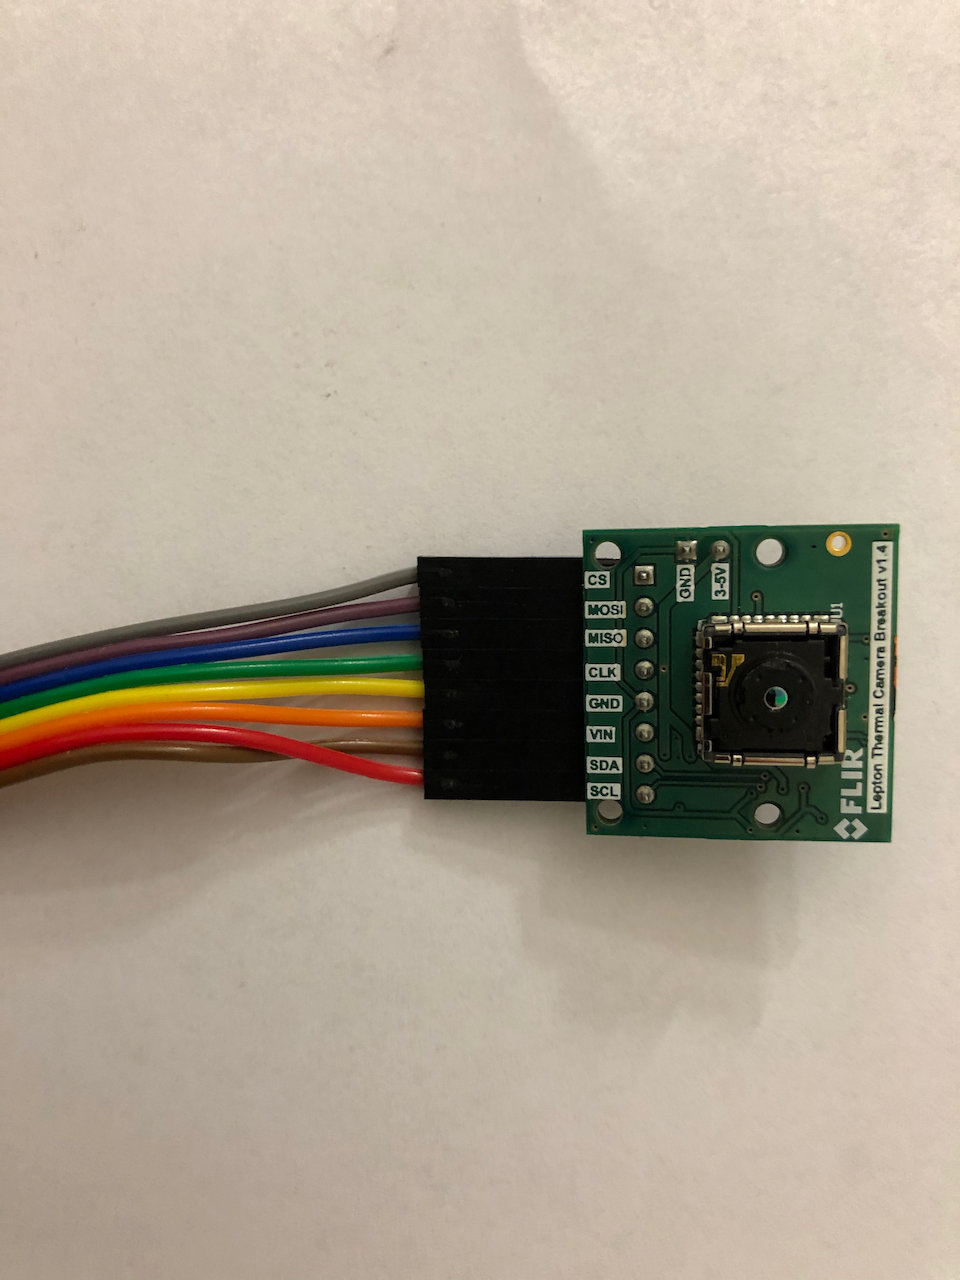
\includegraphics[width=.40\textwidth]{IMG_0361.jpg}} \quad
    \subfloat[][\emph{Top view}.\label{subfig:top.view-gpio}]
        {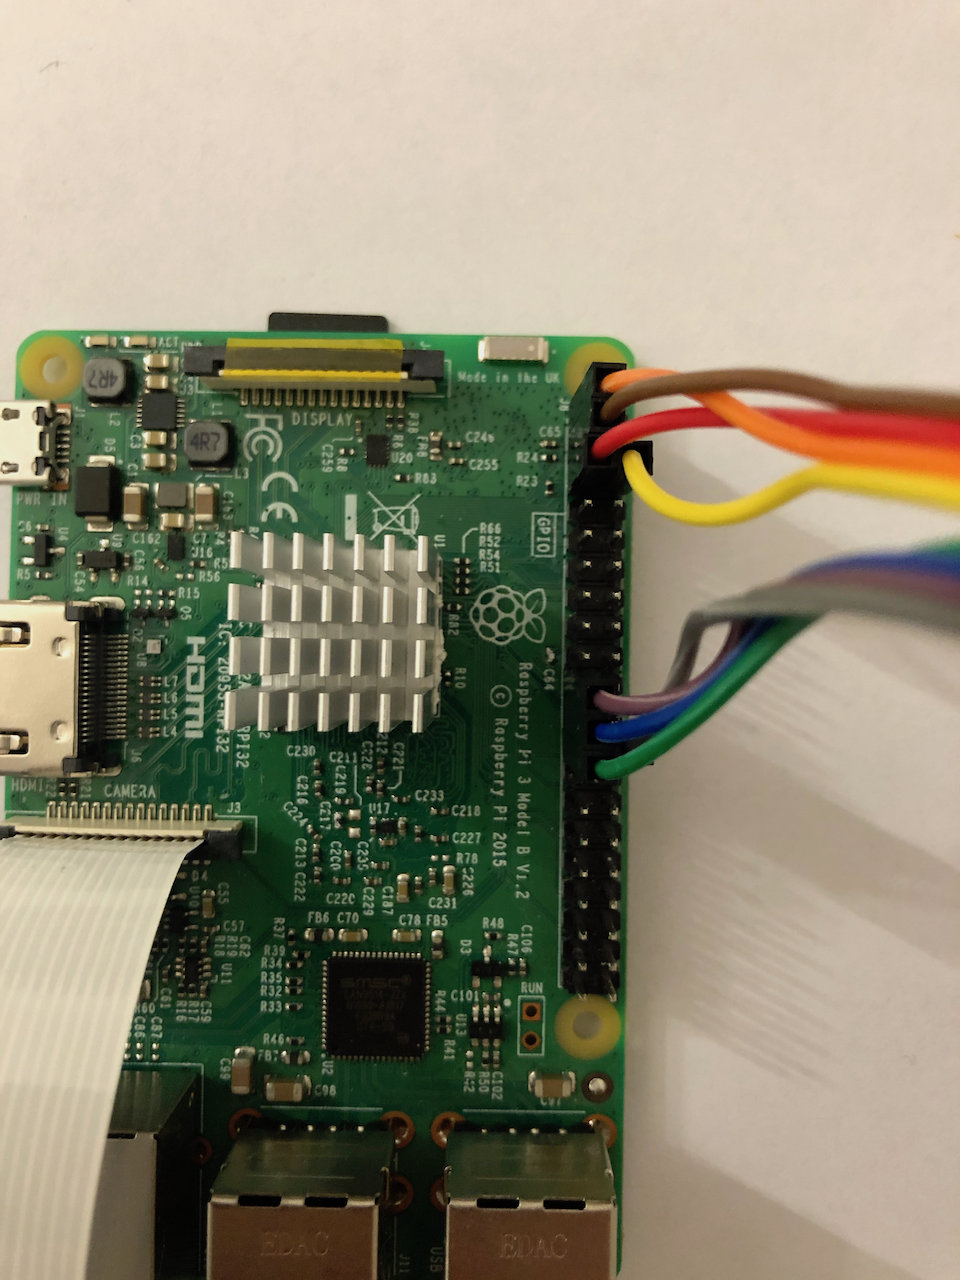
\includegraphics[width=.40\textwidth]{IMG_0362.jpg}} \\
            \subfloat[][\emph{Frontal view}.\label{subfig:front-view-gpio}]
        {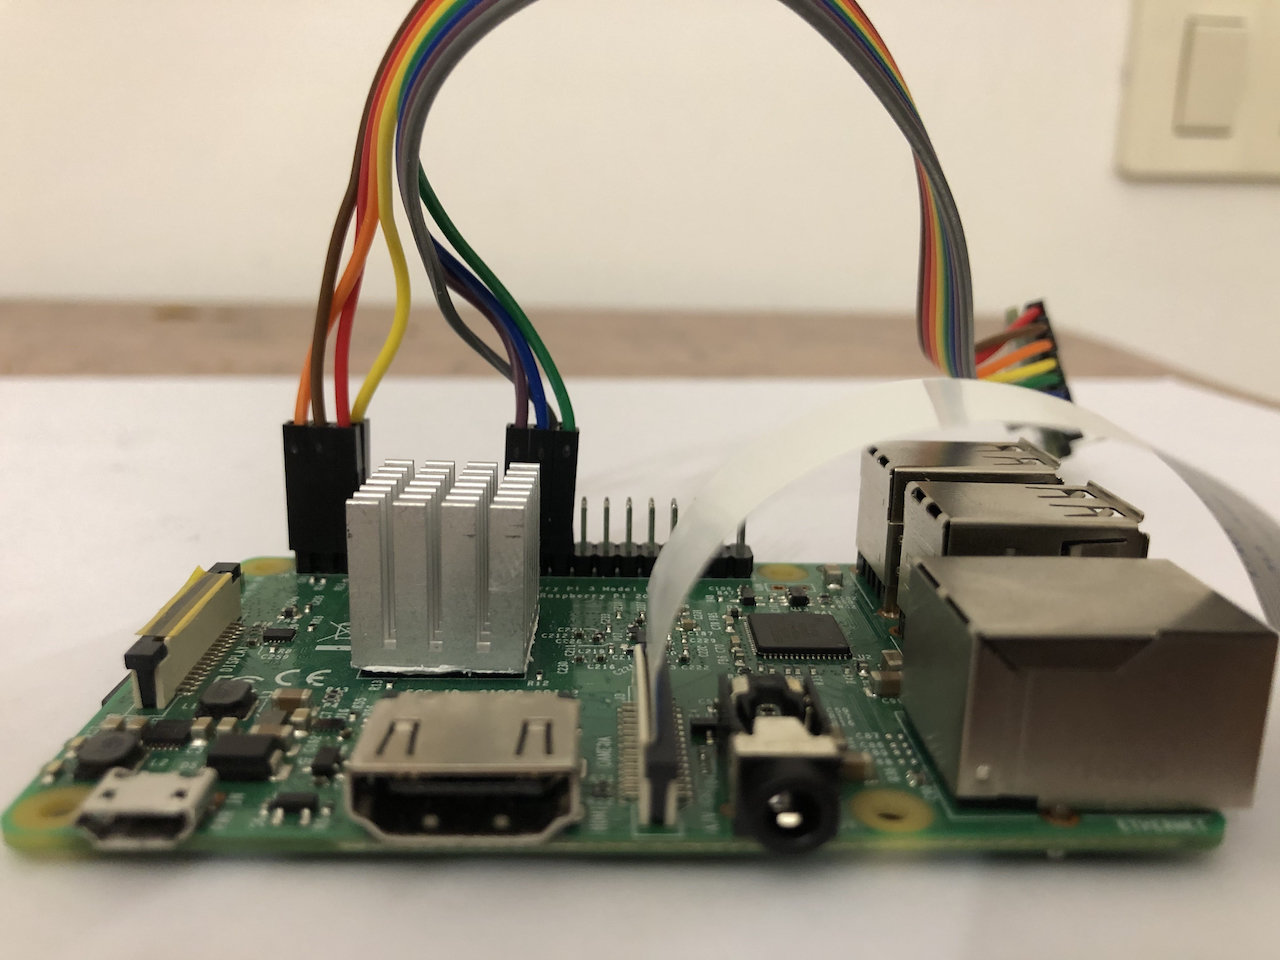
\includegraphics[width=.5\textwidth]{IMG_0360.jpg}}
    \caption{Realization of the connection between the Raspberry Pi 3 GPIO and Break out board}
    \label{fig:brekout-gpio}
\end{figure}
